\chapter{Results}
\label{chap:sidh}
As discussed in previous chapter, we implemented MSFC in ns-3 to see how well it performs in simulated conditions and compare it to other traffic schedulers. We simulate part of wifi network an ISP may manage, since our scheduler aims to ordinary routers at the "last mile" of the Internet --- a few hops near the customer. We simulate several types of traffic common users generate and evaluate performance of commonly used traffic schedulers. 
% dopisat uvod k vysledkom mby

\section{Simulation testbed}

\begin{figure}
	\centering
	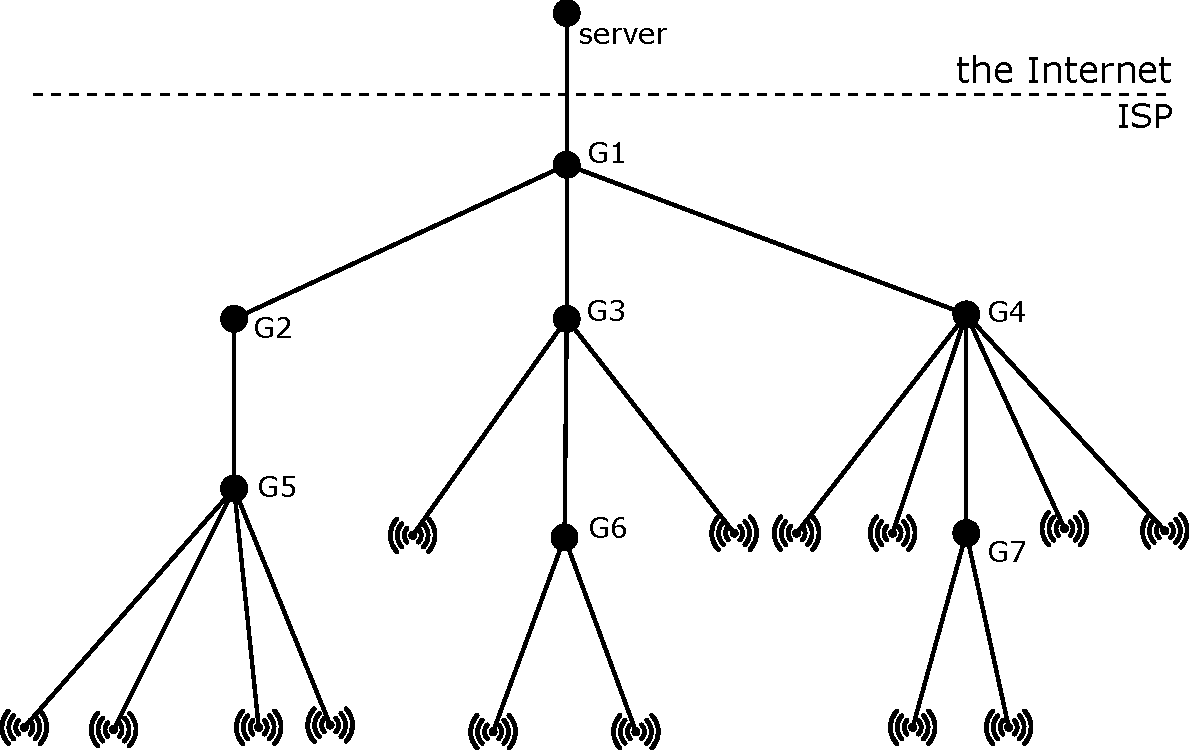
\includegraphics[width=137mm]{drawings/layout}
	\caption{The simulated network topology}
	\label{fig11:sim_layout}
\end{figure}


The simulated network is illustrated in Figure \ref{fig11:sim_layout}. The network is tree-shaped. The topmost node is server, it represents the rest of the Internet. Further, there is part of the infrastructure of an ISP. There are gateway nodes G1-G7. All gateways have 2-5 children. The leafs of this tree are access points (AP) of wireless networks. Finally, 8-12 clients (customers of ISP) are connected to each AP, with the default seed this results in 143 clients. 

Each client is connected to exactly one AP. The clients are connected with 802.11n wifi --- they share the wifi bandwidth. APs and gateways are connected with point-to-point links with 100Mbps bandwidth and 5ms delay. The server is connected to G1 with 200Mbps link with 50ms delay.

The clients download and upload data. All the traffic flows between the server and one of the clients. There are several types of applications that model various behaviour of real-life clients. The types are listed in table \ref{tab01:traffic}. They vary in transport protocol used, size of single packet and data rate at which they generate traffic. The data rate may be constant --- in that case the application generates packets on regular basis (e.g. it sends a packet every 5 milliseconds), or it may be variable.

The applications with variable bit rate turn itself on and off on irregular basis. During off period, it sends zero packets and during on time it sends packets at configured constant rate. The on times and off times are generated randomly --- using normal distribution $\mathcal{N}(1,1)$.

\begin{table}
	\caption{Types of applications}
	\label{tab01:traffic}
	\centering
	
	
	\begin{tabular}{@{}lllllll@{}}
		\toprule
		Name     & Protocol & Data rate & C/VBR   & directions & Packet         & Priority \\ 
		&          &           &         &            & size(B)        & \\ \midrule
		SSH      & TCP      & 1 kbps    & CBR     & both       & 20             & 1        \\
		VoIP     & TCP      & 60 kbps   & CBR     & both       & 208            & 2        \\
		Game     & TCP      & 100 kbps  & CBR     & both       & 512            & 1        \\
		TV       & TCP      & 3 Mbps    & CBR     & one        & 1450           & 2        \\
		HTTP     & TCP      & unlimited & VBR     & one        & 256            & 1        \\
		Download & TCP      & unlimited & CBR     & one        & 1450           & 0        \\
		HD stream& UDP      & 10 Mbps   & CBR     & one        & 1450           & 1        \\ \bottomrule
	\end{tabular}
\end{table}



To evaluate MSFC, we ran multiple simulations with different schedulers. Each time, we installed the evaluated scheduler to all nodes (NetDevices) of the simulation. We tested PfifoFast, CoDel, FQ CoDel and MSFC. We have used all schedulers with default parameters. 

We measured total goodput, average delay and jitter. Total goodput is amount of bytes that flows from the server to the clients per second. Average delay is the average time between sending and receiving packet. Jitter is deviation in delay. We use definition of jitter used in \cite{rfc1889}. It computes jitter exponentially weighted moving average:
\begin{align*} 
d &= |NewPacketDelay - PreviousPacketDelay| \\
NewJitter &= OldJitter + \frac{1}{16} (d - OldJitter).
\end{align*}
In other words, $d$ is difference in the delay of two consecutive packets. The jitter from previous packet arrival is then modified slightly towards the delay of the latest packet.

In the first simulation, we assigned priorities to applications according to table \ref{tab01:traffic}. It roughly represents the common application prioritization: VoIP and TV provided by ISP need good QoS the most. On the other hand, download is not QoS sensitive. The results are in table \ref{tab02:results}.




\begin{table}[]
	\centering
	\caption{Results of simulation with priorities set according to table \ref{tab01:traffic}}
	\label{tab02:results}
	\begin{tabular}{lllll}
		\hline
		& PfifoFast & CoDel  & FQ CoDel & MSFC   \\ \hline
		Goodput (kbps)          & 279144    & 277477 & 277375   & 276269 \\
		Delay (ms)              & 1250      & 543    & 156      & 154    \\
		Jitter (ms)             & 27        & 14     & 7        & 7      \\
		Differentiated services &           &        &          &        \\ \hline
	\end{tabular}
\end{table}







\section{Discussion}